\chapter{Data}
\label{chap:three}

Compared to traditional financial data cryptocurrency data tend to be easier
to obtain. However, many data providers have already identified the bussiness 
potential of selling advanced data and have started to monetize them. However,
since some
websites monetize only their APIs we could improvize and obtain data from 
multiple sources and merge them to get to our desired dataset size. We have
desired to use as many relevant variables as possible and we build on
an existing research in the field.
Our dataset can be split into 2 main categories and 4 subcategories.
We utilize the data that describe the overall market trends in the traditional
sense. These data were mostly obtained from \textbf{\href{https://fred.stlouisfed.org/}{https://fred.stlouisfed.org/}}
and from the 
\textbf{\href{https://finance.yahoo.com/markets/}{https://finance.yahoo.com/markets/}} API.
To balance fundamental indicators with speculative side we used \textbf{\href{https://trends.google.com/trends/}{Google Trends}}
and \textbf{\href{https://pageviews.wmcloud.org/}{Wikipedia Page Views}} 
that act as a proxy for market attention about cryptocurrencies in general 
and should help us to model the market hype periods. These explanatory
variables are then used to forecast the price or returns of the specific cryptocurrency
of interest lagged back in time.

\begin{figure}[!h]
    \centering
    \caption{Dataset Variables Overview}
        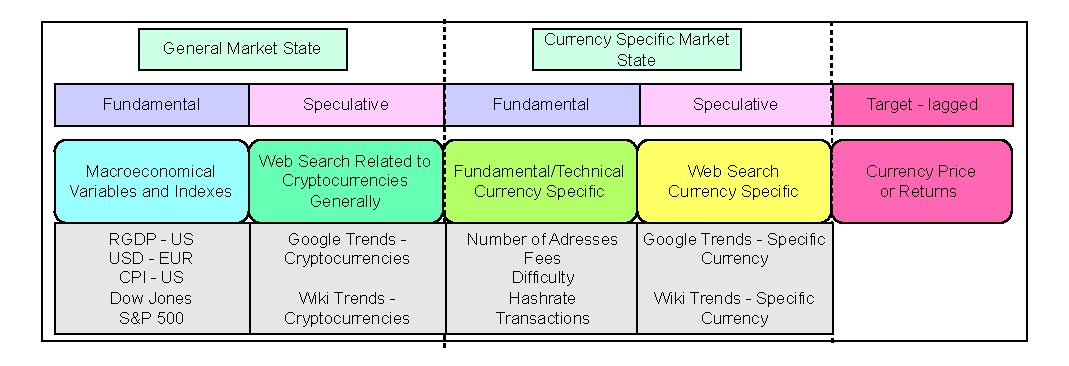
\includegraphics[width=1\textwidth]{Figures/dataset_description.drawio.pdf}
    \label{fig:dataset_description}
\end{figure}


The data were collected between December 2023 to February 2024 varying 
based on
the different sources but they are further shortened to utilize the most
overlapping region between data sources for each unique cryptocurrency.
This results in a time series from 17.9.2014 to 1.11.2022 for Bitcoin, 4.2.2016
to 27.7.2022 for Ethereum ensuring that the end of the series is 
before the change to proof-of-stake algorithm and series from 17.9.2014 to 1.11.2022
for Litecoin. The shifted versions of the datasets are of variable length based
on the forecasting horizon. 
\section{Cryptocurrency Specific Technical Data}




\section{Macroeconomical Data}

As the macroeconomical condition is a cruical factor for investor behaviour 
we decided to include relevant variables that might deliver valuable
insights. We utilize five macroeconomical indicators that affect invesment choices.
Real Gross Domestic product of the United States represents the overall
growth trend of the largest economy in the world with closely related real
gross domestic product per capita telling more about individual resouces which
gives a more complex picture of the state of the US economy despite the 
fact that americans are not the main cryptocurrency investors by nation.
Furthermore we incorporate Consumer Price Index in the United States that
acts as an inflationary measure to capture the spurious correlation between 
prices of USD and BTC-USD exchange rate. M2 base acts as a measure
of dollar liquidity in the circulation. Lastly, the USD-EUR exchange rate
can be thought of as a market state information or its returns as an 
opportunity costs for potential investors. To further adress the problem of spurious
correlation and add the information about growth of other markets we include
various closing prices and other measures of the stock market and other 
investment opportunities. Following is the full description of the macroeconomical
variables used in our work.

\begin{itemize} 
    \item 
\end{itemize}
\section{Web Search Data}

\section{Preprocessing}






Text text text text text text text text text text text text text text text. Text text text text text text text text text text. Text text text text text text text text text text text text text text text. Text text  \citet{Haufler2006}.

Text text text text text text text text text text text text text text text. Text text text text text text text \cite[see, \latinfont{inter alia},][pg.~10]{Haaparanta1996}. 



Text text text text text text text text text text text text text text text. Text text text text text text text text text text. Text text text text text text. Politicians usualy like inward \ac{BTC} and an \ac{MNC} appreciates \ac{FDI} subsidies. Are \acp{MNC} greedy?



To achieve compatibility with PDF/A 2u, your file must not include links to external fonts, audio, video, or scripts. On the other hand, your file must declare each color environment you use, it must include all the pictures/figures either in jpeg or PDF/A 2u format, used fonts compliant under Unicode (your file cannot use any external fonts), and it must include meta-data in XMP format.


Most troubleshooting comes from the conversion of figures to compliant formats. You can convert from simple PDF using Adobe Acrobat:



But most of the vector graphics gets distorted to lower quality in Adobe (like pictures in pdfs generated from Stata, unless jpeg is sufficient for you). You can also use GhostScript, the conversion tool is provided by courtesy of the Faculty of Mathematics and Physics at

\vspace{0.5cm}
\textbf{\href{https://kam.mff.cuni.cz/pdfix/}{https://kam.mff.cuni.cz/pdfix/}}
\vspace{0.5cm}

Text text text text text text.\footnote{Text text text text text text text text text text text text text text text. Text text text text text text text text text text. Text text text text text text.} Font of Latin phrases should be consistent: Furthermore, there is no \latinfont{ex post} price effect, all things being equal (\latinfont{ceteris paribus}). This is \latinfont{per se} truth.

\begin{figure}[!htbp]
\begin{center}
\caption{Market equilibrium}
\label{fig:supply}
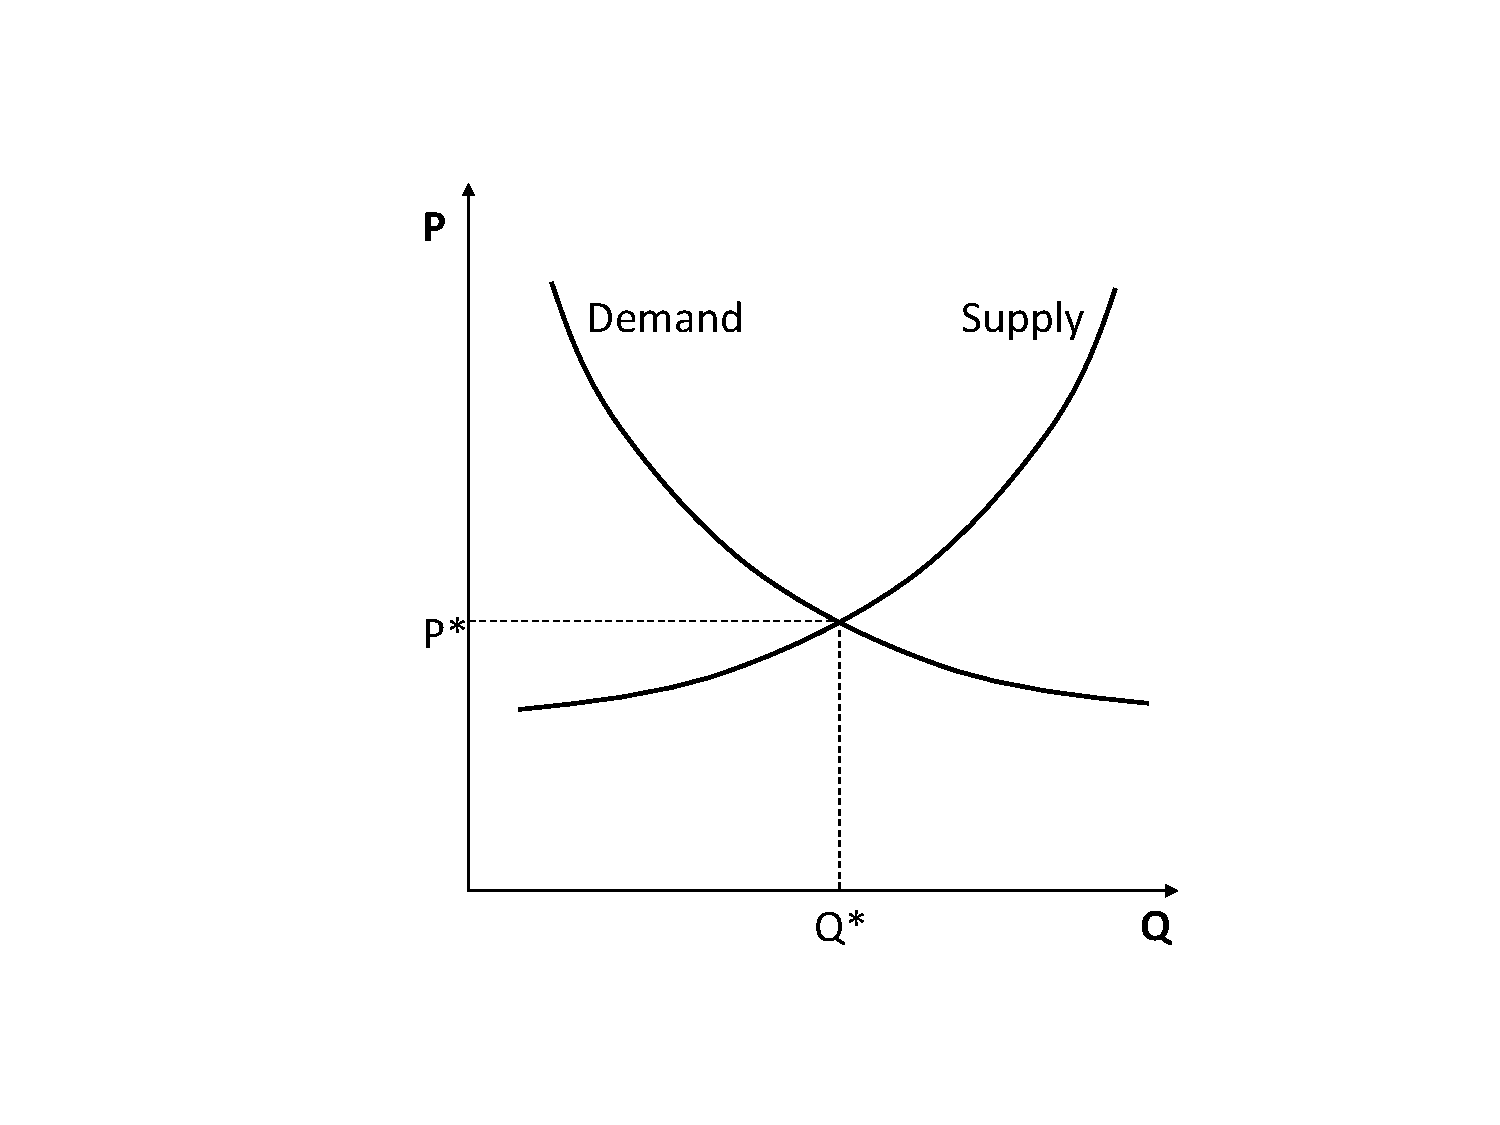
\includegraphics[width=60mm]{Figures/supplydemand}
\end{center}\vspace{-0.5cm}
\begin{source}\cite{Haufler2006}.\end{source}
\end{figure}

Look at the \autoref{fig:supply}. Text text text text text text text text text text. Text text text text text text. Text text text text text text text text text text. Text text text text text text text text text text.





If you use Stata, you might want to check the \texttt{sutex}, \texttt{outtable}, \texttt{outtex}, and \texttt{estout} tools, which help you with exporting Stata tables to \LaTeX{}.


\begin{table}[!htbp]
\begin{center}
	\caption[Calibration table]{Model's predictions}\label{tab:values}
\begin{tabular}{lrrrrrrrrrr}
\toprule
\textit{Case} &        $Y_1$ &        $Y_2$ &  $\tau_1$ &  $\tau_2$ &          $a$ &          $n$\\
\midrule
CR---Slovakia &       10.9 &         10 &       0.24 &       0.19 &          1,000 &       2.16\\

CR---Poland &       13.3 &         12 &       0.24 &       0.19 &          1,000 &       0.38\\

CR---Hungary &       10.4 &          8 &       0.24 &       0.16 &          1,000 &        1.10\\
\bottomrule
\end{tabular}  
\end{center}
\begin{source} If the source is author himself (like a calculation output), this line is redundant.\end{source}
\end{table}

Text text text text text text text text text text text text text text text. Text text text text text text text text text text. Text text text text text text. Text text text text text text text text text text. Text text text text text text text text text text.



Text text text text text text text text text text text text text text text. Text text text text text text text text text text. Text text text text text text. Text text text text text text text text text text. Text text text text text text text text text text. Let us make a box:

\begin{figure}[!htbp]
\begin{center}
\caption{Boxy's example}\label{box:values}
\begin{boxeditemize}
	\item Welcome to Boxy paragraph. 
We sincerely hope you will
all enjoy the show.
	\item
Welcome to Boxy paragraph.
We sincerely hope you will
all enjoy the show.
	\item 
Welcome to Boxy paragraph.
We sincerely hope you will
all enjoy the show.
\end{boxeditemize}
\end{center}
\begin{source}\cite{Haaparanta1996}\end{source}
\end{figure}

Text text text text text text text text text text text text text text text. Text text text text text text text text text text. Text text text text text text. Text text text text text text text text text text. Text text text text text text text text text text.


\begin{defin}[My original definition]\label{de:definice1}
This is a definition.
\end{defin}

\begin{ass}[My realistic assumption]\label{as:predpoklad1}
This is an assumption.
\end{ass}

\begin{prop}[My clever proposition]\label{pr:veta1}
This is a proposition.
\end{prop}

\begin{lemma}[My useful lemma]\label{le:lemma1}
This is a lemma.
\end{lemma}

\begin{exam}\label{ex:priklad1}
This is an example.
\end{exam}

\begin{proof}
This is a proof.
\end{proof}



Text text text text text text text text text text text text text text text. Text text text text text text text text text text. Text text text text text text. Text text text text text text text text text text. Text text text text text text text text text text.

    \[ U = \underbrace{\int_0^{\infty} \frac{1}{1-\sigma}\left(C^{1-\sigma} -1 \right) e^{-\rho t} \ud t}_\text{meaning of life} \]


Text text text text text text text text text text text text text text text. Text text text text text text text text text text. Text text text text text text. Text text text text text text text text text text. Text text text text text text text text text text.
\begin{equation}\label{eq:rovnice1}
    U = \int_0^{\infty} \overbrace{ \frac{1}{1-\sigma}\left(C^{1-\sigma} -1 \right)}^\text{instantaneous utility} e^{-\rho t} \ud t
\end{equation}


Text text text text text text text text text text text text text text text. Text text text text text text text text text text. Text text text text text text. Text text text text text text text text text text. Text text text text text text text text text text.

\begin{equation}\label{eq:rovnice2}
    \mat{A} = \mat{B} + \mat{C}
\end{equation}


\begin{itemize}
    \item to literature~\citep[pg.~10]{Bjorvatn2006} 	
            or~\citet[pg.~10]{Haufler2006},
    \item to~\autoref{fig:supply},														%or use \autoref
    \item see~\autoref{tab:values},
    \item to~\autoref{rovnice},
    \item to~\defref{de:definice1}, to~\proref{pr:veta1},
            \exaref{ex:priklad1}, 
    \item to equations like this: see~\eqref{eq:rovnice1}.
\end{itemize}


You can input a source code like this:
\begin{matlab}{.9\linewidth}{dgreen}
    omega = 1;
    syms zeta;
    jmn = [1 2*zeta*omega omega^2];
    figure(1);
        for zeta = 1E-5 : 0.2 : 1+1E-12
            G = tf(omega^2,subs([1 2*zeta*omega omega^2]));
            bode(G); hold on;
        end
    legend('\zeta = 0','\zeta = 0,2','\zeta = 0,4','\zeta = 0,6',');
\end{matlab}
Should you prefer a different font size, redefine file \texttt{Styles/Mystyle.sty}.


Usually you should not use the first person singular (I) in your text, write we instead. As a general recommendation, use the first person sparsely, sometimes it can be replaced by a phrase like ``This work presents \ldots.''

Text text text text text text text text text text text text text text text. Text text text text text text text text text text. Text text text text text text. Text text text text text text text text text text. Text text text text text text text text text text. Text text text text text text \citep{Haufler2006}. Let us make two paragraphs:

\paragraph{Proin} Text text text text text text text text text text text text text text text. Text text text text text text text text text text. Text text text text text text. Text text text text text text text text text text. Text text text text text text text text text text.
Text text text text text text text text text text text text text text text. Text text text text text text text text text text. Text text text text text text. And a subparagraph:
\subparagraph{Velit} Text text text text text text text text text text text text text text text. Text text text text text text text text text text. Text text text text text text. Text text text text text text text text text text. Text text text text text text text text text text.

